\documentclass[journal, a4paper]{IEEEtran}
%\usepackage{natbib}
\usepackage{graphicx}

\usepackage{hyperref}
\hypersetup{
	colorlinks=true,
	linkcolor=blue,
	filecolor=magenta,      
	urlcolor=cyan,
}

% some very useful LaTeX packages include:

%\usepackage{cite}      % Written by Donald Arseneau
                        % V1.6 and later of IEEEtran pre-defines the format
                        % of the cite.sty package \cite{} output to follow
                        % that of IEEE. Loading the cite package will
                        % result in citation numbers being automatically
                        % sorted and properly "ranged". i.e.,
                        % [1], [9], [2], [7], [5], [6]
                        % (without using cite.sty)
                        % will become:
                        % [1], [2], [5]--[7], [9] (using cite.sty)
                        % cite.sty's \cite will automatically add leading
                        % space, if needed. Use cite.sty's noadjust option
                        % (cite.sty V3.8 and later) if you want to turn this
                        % off. cite.sty is already installed on most LaTeX
                        % systems. The latest version can be obtained at:
                        % http://www.ctan.org/tex-archive/macros/latex/contrib/supported/cite/

\usepackage{graphicx}   % Written by David Carlisle and Sebastian Rahtz
                        % Required if you want graphics, photos, etc.
                        % graphicx.sty is already installed on most LaTeX
                        % systems. The latest version and documentation can
                        % be obtained at:
                        % http://www.ctan.org/tex-archive/macros/latex/required/graphics/
                        % Another good source of documentation is "Using
                        % Imported Graphics in LaTeX2e" by Keith Reckdahl
                        % which can be found as esplatex.ps and epslatex.pdf
                        % at: http://www.ctan.org/tex-archive/info/

%\usepackage{psfrag}    % Written by Craig Barratt, Michael C. Grant,
                        % and David Carlisle
                        % This package allows you to substitute LaTeX
                        % commands for text in imported EPS graphic files.
                        % In this way, LaTeX symbols can be placed into
                        % graphics that have been generated by other
                        % applications. You must use latex->dvips->ps2pdf
                        % workflow (not direct pdf output from pdflatex) if
                        % you wish to use this capability because it works
                        % via some PostScript tricks. Alternatively, the
                        % graphics could be processed as separate files via
                        % psfrag and dvips, then converted to PDF for
                        % inclusion in the main file which uses pdflatex.
                        % Docs are in "The PSfrag System" by Michael C. Grant
                        % and David Carlisle. There is also some information
                        % about using psfrag in "Using Imported Graphics in
                        % LaTeX2e" by Keith Reckdahl which documents the
                        % graphicx package (see above). The psfrag package
                        % and documentation can be obtained at:
                        % http://www.ctan.org/tex-archive/macros/latex/contrib/supported/psfrag/

%\usepackage{subfigure} % Written by Steven Douglas Cochran
                        % This package makes it easy to put subfigures
                        % in your figures. i.e., "figure 1a and 1b"
                        % Docs are in "Using Imported Graphics in LaTeX2e"
                        % by Keith Reckdahl which also documents the graphicx
                        % package (see above). subfigure.sty is already
                        % installed on most LaTeX systems. The latest version
                        % and documentation can be obtained at:
                        % http://www.ctan.org/tex-archive/macros/latex/contrib/supported/subfigure/

\usepackage{url}        % Written by Donald Arseneau
                        % Provides better support for handling and breaking
                        % URLs. url.sty is already installed on most LaTeX
                        % systems. The latest version can be obtained at:
                        % http://www.ctan.org/tex-archive/macros/latex/contrib/other/misc/
                        % Read the url.sty source comments for usage information.

%\usepackage{stfloats}  % Written by Sigitas Tolusis
                        % Gives LaTeX2e the ability to do double column
                        % floats at the bottom of the page as well as the top.
                        % (e.g., "\begin{figure*}[!b]" is not normally
                        % possible in LaTeX2e). This is an invasive package
                        % which rewrites many portions of the LaTeX2e output
                        % routines. It may not work with other packages that
                        % modify the LaTeX2e output routine and/or with other
                        % versions of LaTeX. The latest version and
                        % documentation can be obtained at:
                        % http://www.ctan.org/tex-archive/macros/latex/contrib/supported/sttools/
                        % Documentation is contained in the stfloats.sty
                        % comments as well as in the presfull.pdf file.
                        % Do not use the stfloats baselinefloat ability as
                        % IEEE does not allow \baselineskip to stretch.
                        % Authors submitting work to the IEEE should note
                        % that IEEE rarely uses double column equations and
                        % that authors should try to avoid such use.
                        % Do not be tempted to use the cuted.sty or
                        % midfloat.sty package (by the same author) as IEEE
                        % does not format its papers in such ways.

\usepackage{amsmath}    % From the American Mathematical Society
                        % A popular package that provides many helpful commands
                        % for dealing with mathematics. Note that the AMSmath
                        % package sets \interdisplaylinepenalty to 10000 thus
                        % preventing page breaks from occurring within multiline
                        % equations. Use:
%\interdisplaylinepenalty=2500
                        % after loading amsmath to restore such page breaks
                        % as IEEEtran.cls normally does. amsmath.sty is already
                        % installed on most LaTeX systems. The latest version
                        % and documentation can be obtained at:
                        % http://www.ctan.org/tex-archive/macros/latex/required/amslatex/math/



% Other popular packages for formatting tables and equations include:

%\usepackage{array}
% Frank Mittelbach's and David Carlisle's array.sty which improves the
% LaTeX2e array and tabular environments to provide better appearances and
% additional user controls. array.sty is already installed on most systems.
% The latest version and documentation can be obtained at:
% http://www.ctan.org/tex-archive/macros/latex/required/tools/

% V1.6 of IEEEtran contains the IEEEeqnarray family of commands that can
% be used to generate multiline equations as well as matrices, tables, etc.

% Also of notable interest:
% Scott Pakin's eqparbox package for creating (automatically sized) equal
% width boxes. Available:
% http://www.ctan.org/tex-archive/macros/latex/contrib/supported/eqparbox/

% *** Do not adjust lengths that control margins, column widths, etc. ***
% *** Do not use packages that alter fonts (such as pslatex).         ***
% There should be no need to do such things with IEEEtran.cls V1.6 and later.


% Your document starts here!
\begin{document}

% Define document title and author
	\title{SAVITR- Web service utilising OSM for disaster preparedness and relief operations}
	\author{Ritam Dutt \(14CS30041\), Kaustubh Hiware \(14CS30011\),\\ Avijit Ghosh \(14CH3FP18\), Rameshwar Bhaskaran \(14CS30026\), Nishant Nikhil \(14MA20021\)
	\thanks{}}
	\markboth{}{}
	\maketitle

% Write abstract here
\begin{abstract}
	We present in this paper, an early warning system, called SAVITR. It leverages the vast information hosted on online social media, namely Twitter to forsee, monitor and analyse different disaster and emergency sitautions. It employs natural language processing techniques to infer the location of a tweet from the text in an unsupervised fashion and display it on a map-based interface. 
\end{abstract}

% Each section begins with a \section{title} command
\section{Introduction}
	% \PARstart{}{} creates a tall first letter for this first paragraph
	The onset of online social media and microblogging sites like Facebook and Twitter have revolutionized lives in recent years. It has played a pivotal in the case of emergencies and disaster-related operations like the devastating Nepal Earthquake \footnote{https://en.wikipedia.org/wiki/April\_2015\_Nepal\_earthquake}, Chennai floods \footnote{https://en.wikipedia.org/wiki/2015\_South\_Indian\_floods} and Paris terrorist attacks\footnote{https://en.wikipedia.org/wiki/November\_2015\_Paris\_attacks}.
	The ubiquity of smartphones and the vast popularity of OSM have enabled people to act like social sensors and convey situational information quickly. Consequently, it is not only imperative to process the vast amount of incoming datastream on a real-time basis but also accurately extract relevant information from the unstructured and noisy data.
	
	The work proposes a novel method of extracting locations from the text of English tweets in an unsupervised fashion, in contrast to using the geo-tagged field. The following reasons justify our choice. Firstly, tweets having a valid geo-tagged field are very sparse, especially in a developing country as India. \(0.36\%\). Secondly, geo-tagged tweets might not be an accurate representation of the situation, as we demonstrate shortly. 
	
	We put forward the following research questions in this paper. 
	
	\textbf{RQ1}: What is the performance of the location detection algorithm in terms of coverage and accuracy?
	
\textbf{RQ2:} Is our method accurately able to conform with the real-world scenario? Simply put, is our method reliable?
	
\section{Previous work}	

	A few Information Systems have already been implemented in the USA and other countries for emergency informatics.
	The efficacy of such systems have been demonstrated in a variety of situations. Previous work on real-time earthquake detection in Japan was deployed by \cite{Sakaki} using Twitter users as social sensors. 
	 Simple systems like the Chennai Flood Map \cite{Mapbox} during 2015 Chennai floods have demonstrated the need and utility of Information Systems during emergency events in India. It used a combination of crowdsourcing, open source mapping technologies and contributed to large-scale civic participation. 
	 
	 Likewise, Ushahidi,\cite{Ushahidi} a non-profit crisis-mapping software company utilises the concept of crowdsourcing for social activism and public accountability. Here local observers submit reports using their mobile phones or the internet, while simultaneously creating a temporal and geospatial archive of an ongoing event. Ushahidi has been deployed in situations such as earthquakes in Haiti, Chile, forest fires in Italy and Russia.
	
	The potential of crowdsourcing can be acknowledged from AIDR \cite{AIDR},a platform designed for classifying crisis-related microblogs (tweets). It has been developed by the Qatar Computing Research Institute in collaboration with United Nations Office for Coordination of Humanitarian Affairs (OCHA) and the UN International Children’s Fund (UNICEF).
	
	Our system also works on the same basic principle as the aforementioned ones, information extraction from crowdsourced data. However, unlike \cite{Mapbox} and \cite{Ushahidi}, it is not necessary for the user to explicitly specify the location as a separate field. We intend to infer it from the tweet text, without any prior manual labelling. Consequently the unsupervised algrithm assures that our system is capable of integrating news from different sources. Moreover, unlike other systems which are used during crisis analysis, ours intend to detect the onset of some calamity, by analysing past trends. 
	

\section{Dataset}
We have used the Twitter Streaming API \footnote{https://developer.twitter.com/en/docs}, to collect tweets from 12$^{th}$ September, 2017 to 13$^{th}$ October, 2017, and filtered those containing only dengue or flood. This produced a massive dataset of 317567 tweets collected over a period of 31 days. The tweets were preprocessed to remove duplicate entries and also tweets written in different languages, specified by the "lang" field in the tweet-json object. This resulted in 239269 unique tweets for both categories, floods and dengue. These were further segregated into tagged and untagged based on the presence of a valid location.

Our main aim was to collect and display tweets located only within India's bounding box. Thus, we needed some lexicon to disambiguate whether a place is located inside India and what are it's geographical coordinates. To that end, we scraped the data publicly available from Geonames, \footnote{http://www.geonames.org/} and made a dictionary corresponding to different locations within India. The dictionary has the information of 449973 places within India. However, some places mentioned in this dictionary have high othographic similarity with common English nouns. For example, the word song is a place located in Sikkim, whose coordinates are \(27.24641 'N, 88.50622 'E\).
% Main Part
\section{Methodology}
We now present the methodology employed to infer locations from the tweet as proposed below.
\begin{itemize}
	\item The tweet texts are first preprocessed to remove mentions, urls, hashtags, RTs, unknown characters like \(\&, ...\) and numbers are converted to a NUM tag. Case-folding and stop word removal is not carried out however, since we wish to retain the original text.
	\item We first observe the tweet's corresponding geo-tagged field, if any, and accept only those tweets whose location  corresponds to a region inside of India. However the fraction of such tweets are very less, approximately 0.36\% of the entire dataset.
	
	\item We then obtain the POS tags of the tweet text. $T_{i}$ denotes the POS tag of the $i^{th}$ word of the tweet.  If $T_{i}$ corresponds to a proper noun, we keep on appending words that succeed it, provided they are also proper nouns, delimiters or adjectives. If the word i is followed by a noun which corresponds to village, town, road, hospital, street, etc, we consider the $i^{th}$ word as a viable location. We also consider the tag immediately preceeding the word $T_{i}$ and if it is a preposition which usually preceedes a place or location, like at, in, from, to, near etc, we take that word into consideration as well. Thus we infer from the text proper nouns which conform to locations from their syntactic structure. 
	
	\item We ran a named entity recognizer on the given text and observed those words whose tags correspond to LOC, GPE or FACILITY.
	
	\item We also considered hastags as a possible source of inferring a tweets's location. 
	
	\item Combining the aforementioned techniques, we chose only those words which occur within India's bounding box. 
\end{itemize} . 
The named entity analysis, and POS tag distribution was carried out using SpaCy \footnote{https://spacy.io/} as opposed to the CMU TweeboParser\footnote{http://www.cs.cmu.edu/~ark/TweetNLP/}, due to the heavy processing time of the latter. The TweeboParser was 1000 times slower as opposed to SpaCy. We considered the speed to be a viable trade-off for accuracy since our aim is to deploy a system which would work on a real-time basis and we observed the processing time would be a bottleneck in this regard.

\section{Evaluation}
\subsection{RQ1}
\textbf{What is the performance of the proposed algorithm in terms of accuracy and coverage?}

We define accuracy in terms of F1 score and coverage as the increase in the fraction of tagged tweets.

From the entire set of 239269 tweets, only 3493 were tagged, out of which 869 were from India. This corresponds to a minute proportion of approximately $0.36\%$ of the entire dataset. On the other hand the number of tweets which were successfully tagged using our algorithm was approximately $11.05\%$. This increases the coverage drastically and was able to take into account niche and remote places like Ghatkopar, Pipra village and Kharagpur, besides metropolitan cities like Delhi, Kolkata and Mumbai. 

	\begin{table}[!hbt]
		% Center the table
		\begin{center}
			% Title of the table
			\caption{Coverage of tweets}
			\label{tab:Increase}
			\begin{tabular}{|c|c|c|}
				% To create a horizontal line, type \hline
				\hline
				% To end a column type &
				% For a linebreak type \\
				Stats& Dengue& Flood\\\hline
				Tagged& 14044&13254\\
				Untagged& 65853 & 147785\\
				\%-wise tag& 17.577&8.23\\
				\hline
					
				\hline
			\end{tabular}
		\end{center}
	\end{table}
The relative proportion of tagged tweets for dengue is higher than that of floods as observed in Table~\ref{tab:Increase}. This discrepancy arises since dengue is a niche and more specialised topic as opposed to the other. 
Consequently while streaming for floods, we obtained irrelevant tweets of this format \footnote{RT @IndianMillenni1: @republic .@iHrithik has proved that hes a real life hero. I hope that love and support for Hrithik floods in afte…}

We have shown a distribution of tagged tweets for the two situations across the timeframe of 31 days.

\begin{figure}[h]
		% Center the figure.
		\begin{center}
			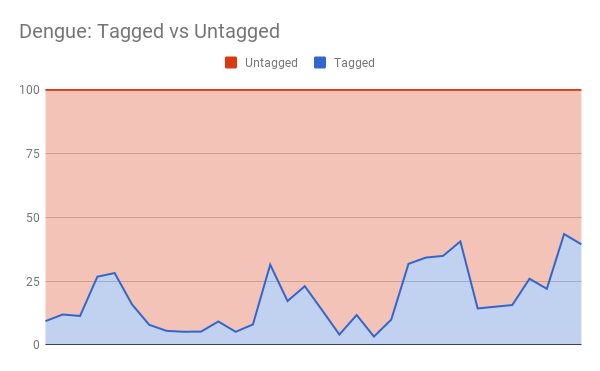
\includegraphics[scale=0.35]{dengue_daily}
			% Create a subtitle for the figure.
			\caption{Proportion of tagged dengue tweets}
			\label{fig:tf_plot}
		\end{center}
\end{figure}
\begin{figure}[h]
	% Center the figure.
	\begin{center}
		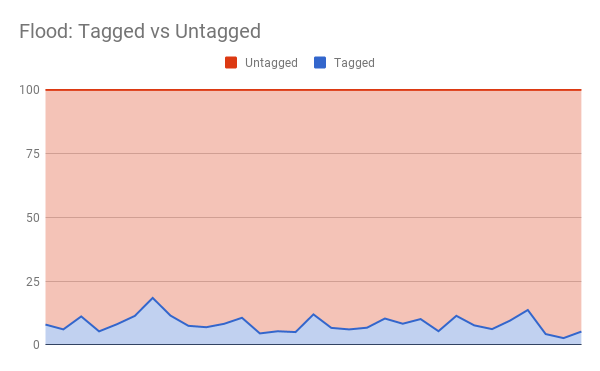
\includegraphics[scale=0.35]{flood_daily}
		% Create a subtitle for the figure.
		\caption{Proportion of tagged flood tweets}
		\label{fig:tf_plot2}
	\end{center}
\end{figure}
 
The important or the more frequently occuring locations are captured in the following word cloud
\begin{figure}[h]
	% Center the figure.
	\begin{center}
		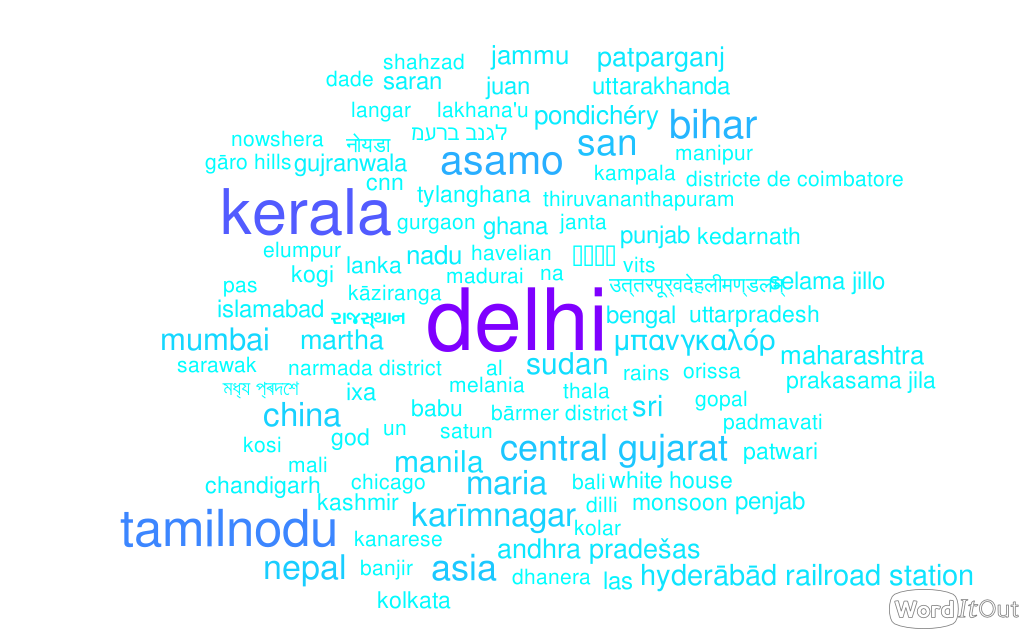
\includegraphics[scale=0.23]{wc}
		% Create a subtitle for the figure.
		\caption{Most frequently occuring cities}
		\label{fig:word_cloud}
	\end{center}
\end{figure}
However we demonstrate that the algorithm was not only able to capture well-known, popular metropolitan locations only but also some remote places inside India, via the Table~\ref{tab:Location}
	\begin{table}[!hbt]
		% Center the table
		\begin{center}
			% Title of the table
			\caption{Coverage of tweets}
			\label{tab:Location}
			\begin{tabular}{|c|c|}
				% To create a horizontal line, type \hline
				\hline
				% To end a column type &
				% For a linebreak type \\
				Type&Location name\\\hline
				
				Frequent& delhi, kerala, tamilnodu, mumbai
				\\
				& assamo, bihar,central gujrat, \\\hline
				Infrequent& indirapuram, ramnagar, hosur, bandra,
				\\
				& tripura,ghaziabad, yamunanagara jila, kharagpur \\
				
				\hline
				
				\hline
			\end{tabular}
		\end{center}
	\end{table}
As observed from the frequency distribution plot, it is evident several rural and remote places occur within India have been identified by the algorithm. The ones in the 
Table~\ref{tab:Location} under the Infrequent category all have a frequency of 1. 
\begin{figure}[h]
	% Center the figure.
	\begin{center}
		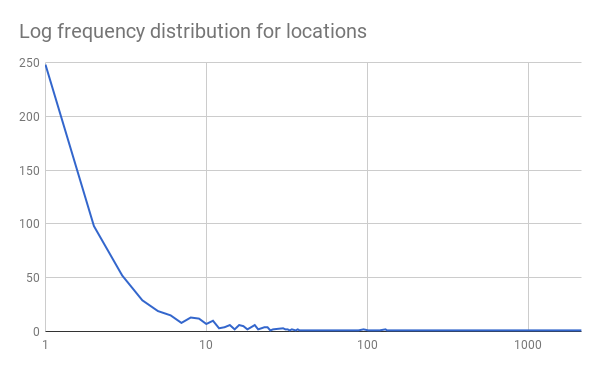
\includegraphics[scale=0.35]{location_freq}
		% Create a subtitle for the figure.
		\caption{Frequency distribution of the freuency of locations }
		\label{fig:freq_dist}
	\end{center}
\end{figure}

It is important to note that there are some invalid locations as well such as potus,
lol, god in the dictionary obtained from Geonames.

We needed to perform an evauation to see the correctness of our algorithm. As mentioned before, we aim to measure the accuracy of the system in terms of precision, recall and F1 score. To that end, we have randomly sampled 200 tagged tweets and another 200 untagged ones. 
We evaluate the precision of the system by observing the tagged tweets and assigning it's relevance if a location within India was mentioned in the tweet. Likewise if it mentions a location not within India, the tweet is deemed invalid. In case a tweet has more than one locations, any one of them is a valid mention. 
Likewise the recall of the system was observed from the untagged tweets. 
The table describes the results in this aspect.

\begin{table}[!hbt]
	% Center the table
	\begin{center}
		% Title of the table
		\caption{Evaluation metrics}
		\label{tab:Evaluation}
		\begin{tabular}{|c|c|c|c|}
			% To create a horizontal line, type \hline
			\hline
			% To end a column type &
			% For a linebreak type \\
			
			&&Actual&\\\hline
			&&Tag&No Tag\\\hline
			Predicted&Tag&152&48\\
			&NoTag&13&187\\		
			\hline
		\end{tabular}
	\end{center}
\end{table}

The precision measured is 0.76, recall is 0.9212 and F1 score is 0.8475

\subsection{RQ2}
\textbf{Is our method accurately able to forsee real-world disaster scenarios? }

In order to analyse the reliability of the system we consider the massive dengue outbreak that plagued India in the fall of 2017. \footnote{https://www.telegraphindia.com/india/dengue-spurt-in-south-182846}. The report, published on 2$^{nd}$ November mentions the plight of the Southern States in the wake of dengue, some of the affected ones being Kerala and Tamil Nadu. We highlight the findings from our data in this aspect.

The number of unique tweets mentioning Kerala and Tamil Nadu were very high. The unnatural reference to these names as opposed to other metropolitan areas like Bangalore or Kolkata is proof that people are referring to these places more. This is evident as we observe the following statistics about Kerala. There were 2204 tweets about Kerala out of which 1960 tweets contain the term dengue. 
This amounts to a 88.89\% overlap.
However most of the data is inferred  from the tweets having Kerala mentioned in their texts. We see some examples of geo-tagged tweets below which talk about Kerala but are posted from other parts of India. This paints an inaccurate description of the situaion. 
	\begin{table}[!hbt]
		% Center the table
		\begin{center}
			% Title of the table
			\caption{Coverage of tweets}
			\label{tab:Kerala}
			\begin{tabular}{|c|c|}
				% To create a horizontal line, type \hline
				\hline
				% To end a column type &
				% For a linebreak type \\
				Tweet Text&Location \\\hline
				Numerous death in Kerala from Dengue,  Chicken guinea,  Malaria&.\\
				@cpimspeak pushed Kerala into a money order econom... & New Delhi\\\hline
				@Bhayankur Hmmm - not rosy in Kerala either ... & New Delhi\\\hline
				Dengue : 5 worst affected states. Scandinavian level HDI state &\\
				Kerala tops the list ... & Bengaluru \\\hline
				45\% of Dengue cases and nearly half the Dengue related deaths&\\
				 in India from Kerala. Too much filth or related to we.. &Bengaluru \\\hline
				@Rameshnair101 @CNNnews18 Dengue cases reported: UP 302,&\\ Kerala 16530
				 .death due to dengue: UP 17, Kerala 28 mortal.. & Kerala\\

				
				\hline
				
				\hline
			\end{tabular}
		\end{center}
	\end{table}

\section{System Description}
\href{https://github.com/JaredHawkins/TweetGeoViz}\\

We started off by developing upon \href{https://github.com/JaredHawkins/TweetGeoViz}{TweetGeoViz}, which was developed in react and nodejs. 
However, due to its bulky nature, the system did not display any results when the database contained over 3 lakh tweets.\\

Owing to ease of control, we decided to port the complete system to Python. The current system, live on \href{http://savitr.herokuapp.com}{savitr.herokuapp.com}, works well at the same number of tweets. It has been built using flask and dash libraries.

\begin{figure}[h!]
	\centering
	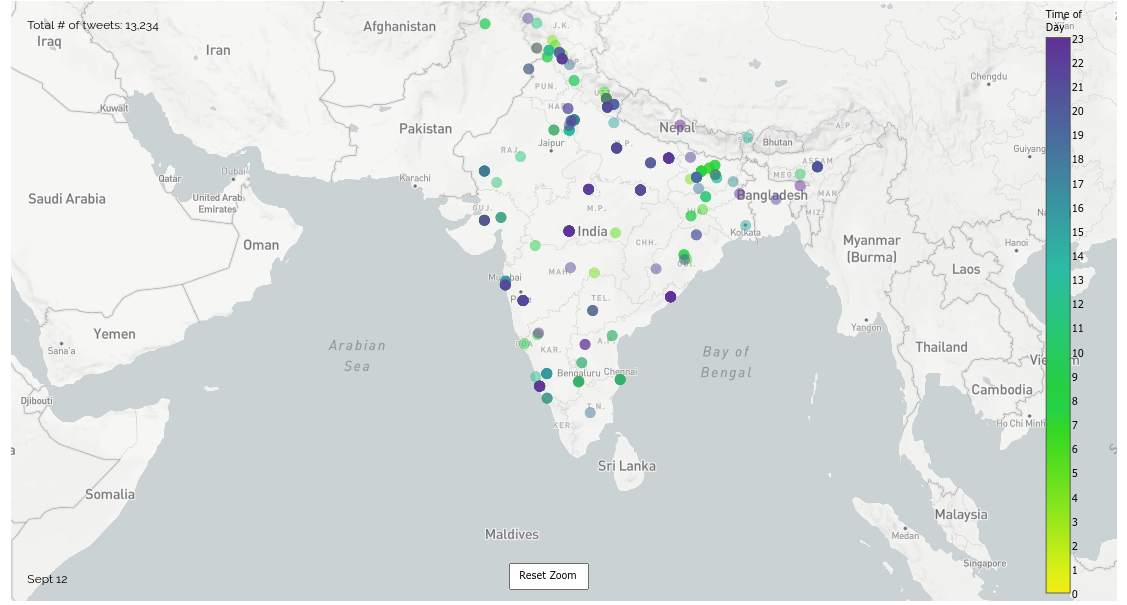
\includegraphics[width=\columnwidth]{map_general.png}
	\caption{ Tweets visualized on India’s map}
	\label{fig:map_general}
\end{figure}


\begin{figure}[h!]
	\centering
	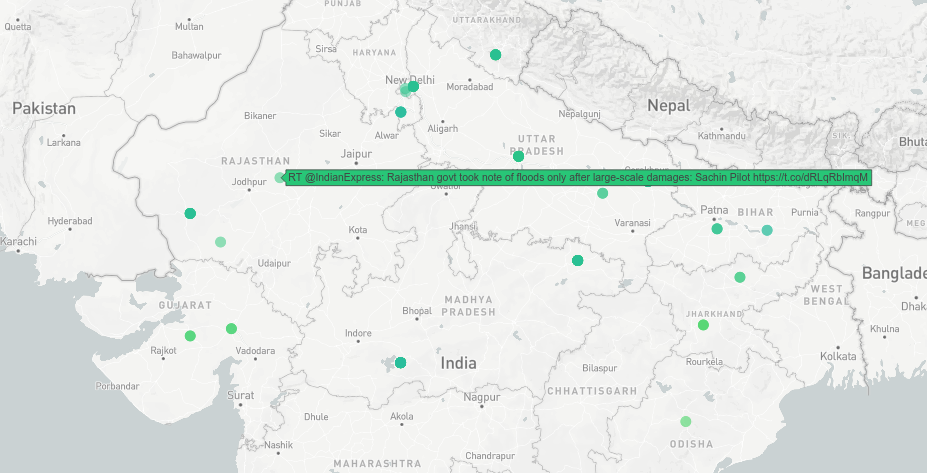
\includegraphics[width=\columnwidth]{map_hovertext.png}
	\caption{Hovering over points reveal tweet text}
	\label{fig:map_hovertext}
\end{figure}


The current system allows the user to search for tweets pertaining certain situations, like floods, dengue, etc. Hovering over a point reveals the tweet text. The possible situations were enlisted beforehand, but it will be possible to search for tweets containing any word.

\begin{figure}[h!]
	\centering
	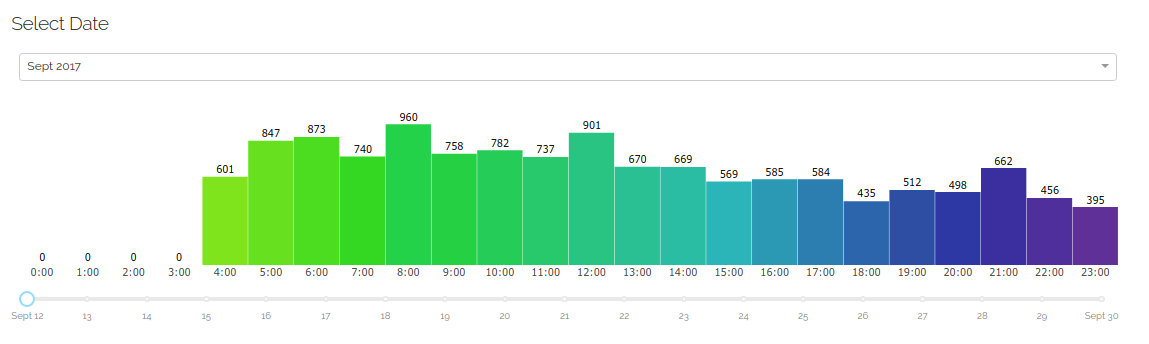
\includegraphics[width=\columnwidth]{bar_chart.png}
	\caption{Tweets sorted by time of posting}
	\label{fig:barchart}
\end{figure}


\begin{figure}[h!]
	\centering
	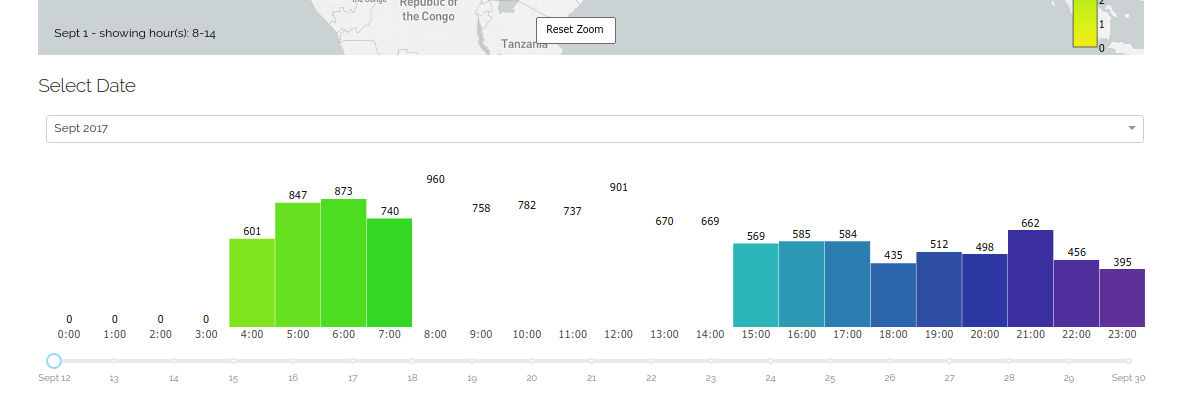
\includegraphics[width=\columnwidth]{bar_chart_specific.png}
	\caption{Crosshair selection of time interval to visualise}
	\label{fig:barchart_specific}
\end{figure}


\begin{figure}[h!]
	\centering
	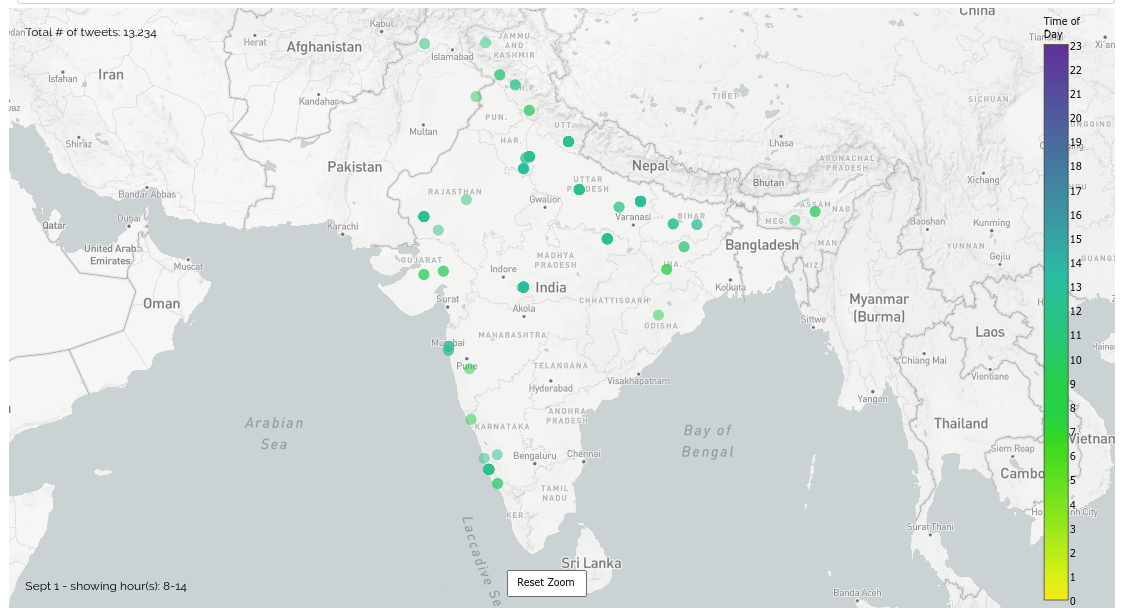
\includegraphics[width=\columnwidth]{map_specific.png}
	\caption{ Tweets for certain time window displayed}
	\label{fig:map_specific}
\end{figure}

\begin{figure}[h!]
	\centering
	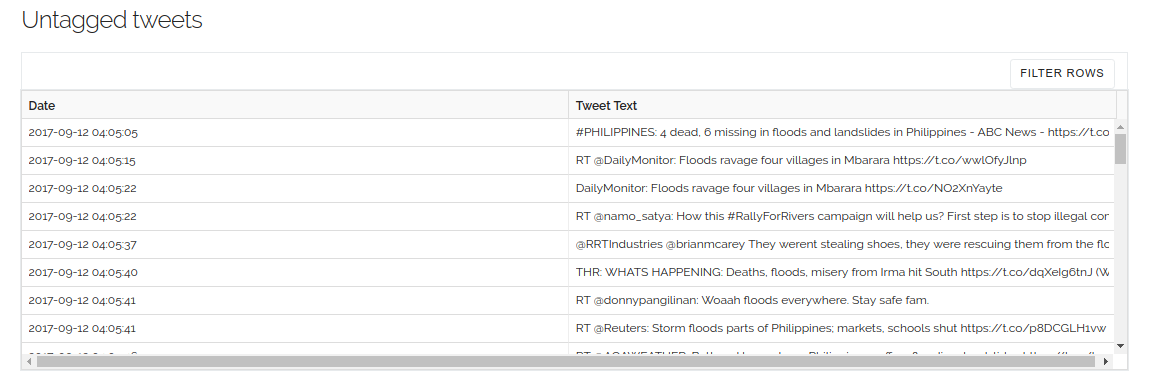
\includegraphics[width=\columnwidth]{untagged.png}
	\caption{Untagged tweets displayed in tabular form at the bottom}
	\label{fig:untagged}
\end{figure}

Untagged tweets are shown separately in tabular format at the very end. At any given instance, the user can see untagged tweets on a certain day. To reduce server strain, the user can only view data spanning 30 days, not more.

Further extensions to be added:
\begin{itemize}
	\item Currently, the data is being displayed from a static file. We will soon be shifting to a database support.
	\item The system will soon be able to visualise tweets spanning multiple days. Currently, the longest duration of tweets visualised in 1 day.
\end{itemize}




\section{Conclusion}
	We have developed an unsupervised algorithm of extracting location information from tweets with a high F1-score of 84.05\%. Moreover the obseravtion mirrored real-life occurences, like the massive dengue outbreak in South India, 2017, which were accurately inferred from the text rather than the geo-tagged location. We have also developed a system that allows for the visual representation and analysis of the potential disaster-scenarios. 

% Now we need a bibliography:
\begin{thebibliography}{5}

	\bibitem{Sakaki}
	Sakaki, Takeshi, Okazaki.
	Earthquake Shakes Twitter Users: Real-time Event Detection by Social Sensors. {\em Proceedings of the 19th International Conference on World Wide Web \(WWW\)},  pp.~851–-860, 2010.
	
	
	\bibitem{Mapbox}
	A.~Ganesh, S.~Bhangar, and S.~Aruna.
	\url{https://osm-in.github.io/flood-map/chennai.html#11/13.0000/80.2000}
	
	\bibitem{Ushahidi}
	\url{https://www.ushahidi.com/}
	
	\bibitem{AIDR}
	\url{http://aidr.qcri.org/}
	%Each item starts with a \bibitem{reference} command and the details thereafter.



\end{thebibliography}

% Your document ends here!
\end{document}